\documentclass[10pt]{article}
\usepackage[utf8]{inputenc}
%\usepackage[T1]{fontenc}
\usepackage{tgbonum}
\usepackage[english]{babel}
\usepackage{graphicx}
\usepackage{amsmath}
\usepackage{amssymb}
\usepackage{hyperref}
\usepackage{epsf}
\usepackage{float}
\usepackage{mathpazo}
\usepackage{pifont}
\usepackage
[
a4paper,% other options: a3paper, a5paper, etc
left=2.2cm,
right=2.2cm,
top=2cm,
bottom=2cm,
]{geometry}
%\geometry{hmargin=3.5cm, vmargin=2.5cm}
\usepackage{fancyhdr}
\pagestyle{fancy}
\fancyhf{}
\rfoot{\thepage}
\renewcommand{\headrulewidth}{0pt}
\usepackage{color}
\usepackage{graphicx}
\usepackage{wrapfig}
\usepackage{graphicx}
\usepackage{multicol}
\usepackage{enumitem}
\usepackage{xcolor}
\usepackage{framed}
\usepackage{bm}
\definecolor{shadecolor}{RGB}{139, 231, 3}
\usepackage{epigraph}

\usepackage{tcolorbox}
\definecolor{mycolor}{rgb}{0.122, 0.435, 0.698}

\newtcbox{\mb}{nobeforeafter,colframe=mycolor,colback=mycolor!10!white,boxrule=0.5pt,arc=4pt,
  boxsep=0pt,left=6pt,right=6pt,top=3pt,bottom=3pt,tcbox raise base}

\usepackage{eso-pic}
\newcommand\BackgroundPic{%
\put(-0,-150){%
\parbox[b][\paperheight]{\paperwidth}{%
\vfill
\centering
\includegraphics[width=\paperwidth,%
keepaspectratio]{plots/foret-de-soignes.jpg}%
\vfill
}}}

\usepackage[T1]{fontenc}

\usepackage{anyfontsize}
\usepackage{t1enc}
\newcommand{\heart}{\ensuremath\varheartsuit}
\usepackage{tikz}
\usetikzlibrary{positioning}
\usepackage{charter}

\setlength{\parskip}{0.6em}
\setlength{\parindent}{0cm}

\begin{document}


  \begin{center}
%\textcolor{lgray}
    \vskip-5em

    \hfill
    \fontsize{10}{10}\selectfont {\textit{Bruxelles, July 2020}}
    \vskip2ex
	\vspace{5ex}
    \fontsize{16}{10}\selectfont {Steady-state conduction in an insulated rod}
    
      \vspace{0.2ex}
      
\fontsize{16}{10}\selectfont {with internal heat production}

  \noindent%
    
\vskip1ex

{\rule{\textwidth}{0.1pt}}

\end{center}
  
    \fontsize{7}{10}\selectfont {This work is licensed under the Creative Commons Attribution-NonCommercial-ShareAlike 4.0 International (CC BY-NC-SA 4.0) license.}

\vspace{5mm}


%%% HEADER END -----------------------------------------------------------
% ------------------------------------------------------------------------

\fontsize{14}{10}\selectfont {Kamila Zdybał}

\fontsize{8}{10}\selectfont {\textit{Université libre de Bruxelles, kamila.zdybal@ulb.ac.be}}

\fontsize{8}{10}\selectfont {\textit{camillejr.github.io/science-docs, kamila.zdybal@gmail.com}}

\vspace{5mm}

This tutorial is based on a Jupyter notebook that can be accessed \href{https://github.com/camillejr/fluid-dynamics-and-transport-phenomena/blob/master/transport-phenomena-with-Python/code/example-heat-transfer-in-a-rod.ipynb}{\textbf{here}}.

\section*{Analytic solution}

In this example, we will derive a one-dimensional temperature distribution function $T(x)$ for a steady-state heat conduction in a straight rod of length $L$. We also assume that there is an internal heat production $Q_p$ ($W/m^3$) at every point inside the rod volume. This may for instance simulate heating up of a wire due to electrical current. The rod is perfectly insulated along its length and it looses heat only through its endpoints which in a steady-state case are kept at a fixed temperature $T_0$. The material from which the rod is made has thermal conductivity $\lambda$ ($\frac{W}{mK}$).

Let's start with writing out the energy balance for an infinitesimal control volume. The control volume will be a slice from the rod of length $dx$. This is presented in figure below:
\begin{figure}[H]
\centering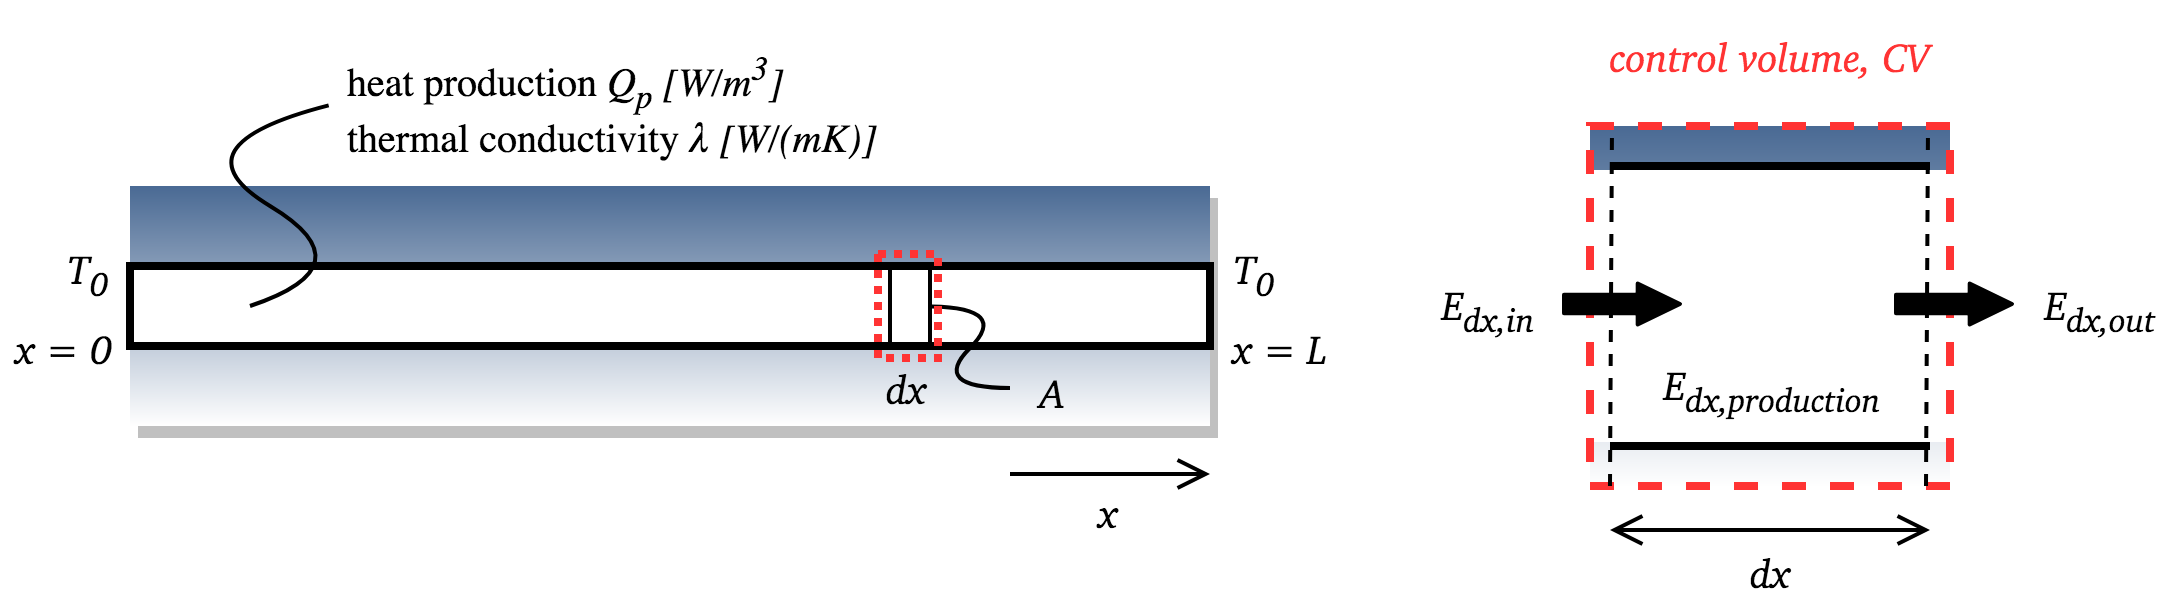
\includegraphics[width=16cm]{plots/cond-rod.png}
\caption{Conduction in a lengthwise-insulated rod with internal heat production.}
\label{fig:conduction}
\end{figure}
The energy balance for the rod element $dx$ is:
\begin{equation}
\frac{dE_{dx}}{dt} = E_{dx, in} - E_{dx, out} + E_{dx, production}
\end{equation}
Note that $E_{dx, in}$, $E_{dx, out}$ and $E_{dx, production}$ are energies per unit time and so have the units of $W$.

The heat flux $\phi$ ($W$) can be modeled using the Fourier's law for one-dimensional heat conduction:

\begin{equation}
\phi = \lambda A \Big(- \frac{dT}{dx} \Big)
\label{eq:fourier}
\end{equation}

where $\lambda$ is the thermal conductivity and is a property of the material, $A$ is the rod's cross-sectional area and $\frac{dT}{dx}$ is a temperature gradient which is the "driving force" for thermal energy transport.

Hence:

\begin{equation}
E_{dx, in} = \lambda A \Big(- \frac{dT}{dx} \Big)_x
\end{equation}

\begin{equation}
E_{dx, out} = \lambda A \Big(- \frac{dT}{dx} \Big)_{x + dx}
\end{equation}

The energy per unit time coming from the heat production can be written as $Q_p$ multiplied by the volume of the slice $dx$:

\begin{equation}
E_{dx, production} = Q_p A dx
\end{equation}

In the steady-state $\frac{dE}{dt} = 0$ and the energy balance becomes:

\begin{equation}
\lambda A \Big(- \frac{dT}{dx} \Big)_x - \lambda A \Big(- \frac{dT}{dx} \Big)_{x + dx} + Q_p A dx = 0
\end{equation}

Simplifying the above energy balance we get:

\begin{equation*}
\frac{\Big(\frac{dT}{dx} \Big)_{x + dx} - \Big(\frac{dT}{dx} \Big)_x  }{dx} = - \frac{Q_p}{\lambda}
\end{equation*}

It is interesting to note here that we have lost the dependence on the cross-sectional surface area of the rod.

If we now substitute some function $f(x) = \frac{dT}{dx}$ we notice that we have:

\begin{equation*}
\frac{f(x + dx) - f(x)}{dx} = - \frac{Q_p}{\lambda}
\end{equation*}

in other words:

\begin{equation}
\frac{df(x)}{dx} = - \frac{Q_p}{\lambda}
\end{equation}

With the above substitution, the differential equation that we are about to solve becomes:

\begin{equation}
\frac{d^2T}{dx^2} = - \frac{Q_p}{\lambda}
\end{equation}

Applying the boundary conditions from both ends of the rod, the solution to the above differential equation is:

\begin{equation}
T(x) = - \frac{Q_p}{2 \lambda} (x^2 - Lx) + T_0
\label{eq:solution}
\end{equation}

\subsection*{Remark on the problem dimensionality}

Note that even though the heat flow was assumed to be one-dimensional in this exercise, it does not mean that the geometry of the problem needs to be one-dimensional. In fact, we assumed the rod to be a three-dimensional object having length and a cross-sectional area. Rather, the one-dimensionality of the problem means that it is practical to assume only one of the three directions as an important direction for heat transport. Since the rod was perfectly insulated along its length, the temperature gradient along directions perpendicular to the $x$-axis is zero.

\section*{Computational example}

As a computational example we will draw the graph of the temperature distribution in a copper rod $200m$ long with cross-sectional area of $0.01m^2$. We assume that the thermal conductivity for this rod is $400 \frac{W}{m \cdot K}$. The internal heat production in the entire rod is $20 W$.

\begin{figure}[H]
\centering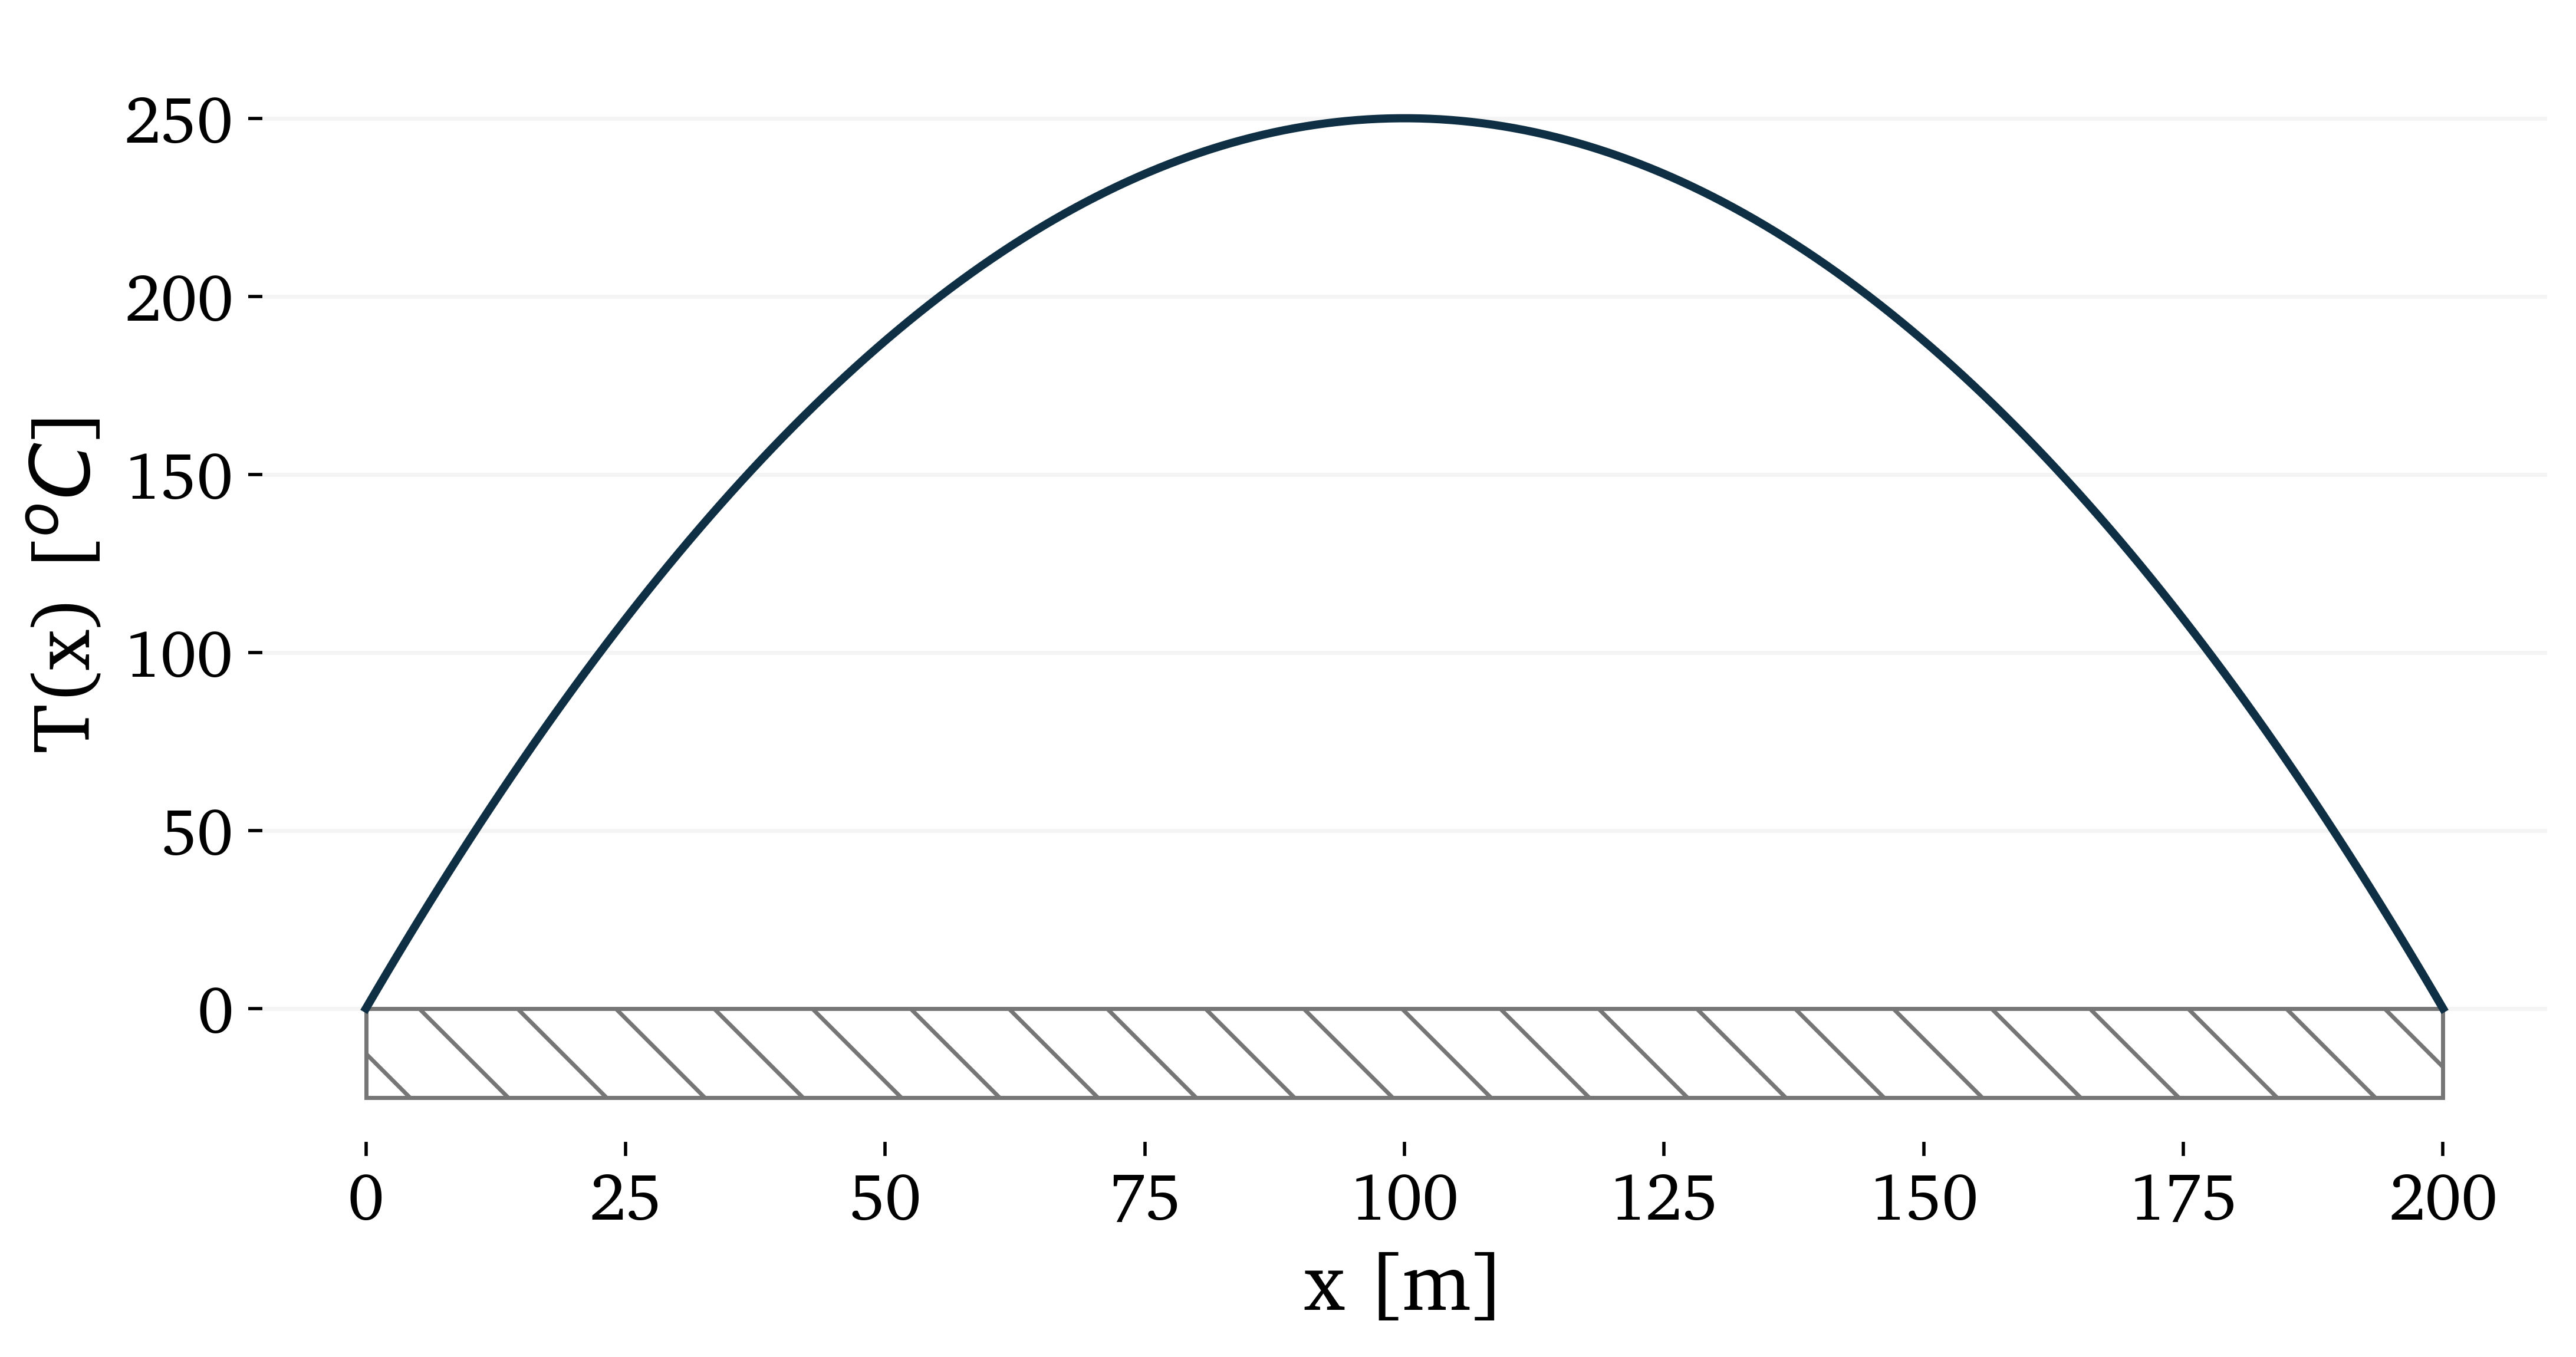
\includegraphics[width=10cm]{plots/example-heat-transfer-in-a-rod-analytic.png}
\caption{Analytic solution for the temperature distribution in a rod.}
\label{fig:analytic-solution}
\end{figure}














\end{document}